\documentclass{standalone} % or article, etc.
\usepackage{tikz}
\usepackage{pgfplots}
\pgfplotsset{compat=1.17} % Adjust if needed

\begin{document}

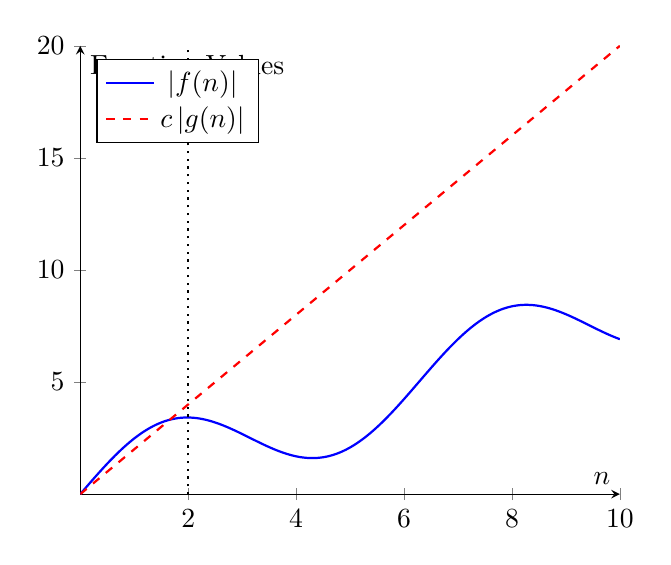
\begin{tikzpicture}
  \begin{axis}[
    axis lines=middle,
    xlabel={$n$},
    ylabel={Function Values},
    xmin=0, xmax=10,
    ymin=0, ymax=20,
    legend style={at={(0.03,0.97)}, anchor=north west}
  ]

    % "Squiggly" function f(n)
    \addplot[
      domain=0:10,
      samples=200,
      smooth,
      thick,
      blue
    ] {0.8*x + 2*sin(deg(x))}; % e.g. 0.8n + 2 sin(n)
    \addlegendentry{$|f(n)|$}

    % Linear bounding function c*g(n)
    \addplot[
      domain=0:10,
      samples=2,  % just plot a straight line with minimal samples
      dashed,
      thick,
      red
    ] {2*x}; % c*g(n) = 2n
    \addlegendentry{$c\,|g(n)|$}

    % Vertical line at n0 = 2
    \draw[dotted, thick] (axis cs:2,0) -- (axis cs:2,20)
        node[above right, black] {$n_0$};

  \end{axis}
\end{tikzpicture}

\end{document}

